\documentclass[10pt,letterpaper]{article}
\usepackage[left=1.8cm, right=1.8cm, top=1cm]{geometry}
\usepackage[utf8]{inputenc}
\usepackage[T1]{fontenc}
\usepackage[spanish]{babel}
\usepackage{amsmath}
\usepackage{amsfonts}
\usepackage{amssymb}
\usepackage{graphicx}
\usepackage{subfigure}
\usepackage{steinmetz}
\usepackage{float}
%\usepackage{circuitikz}

\author{Clase Práctica $\#$8}
\title{Electrónica I}
\date{Aplicaciones de diodos.}

\renewcommand{\sin}{\sen}
\begin{document}
	\maketitle
	
Bibliografía: Electrónica: Teoría de Circuitos y Dispositivos Electrónicos. Robert L. Boylestad y Louis Nashelsky, 10ma ed. Capítulo 2.
\\

1- Trace las formas de onda para $v_o$ en los siguientes circuitos:

\begin{minipage}{8cm}
a)

	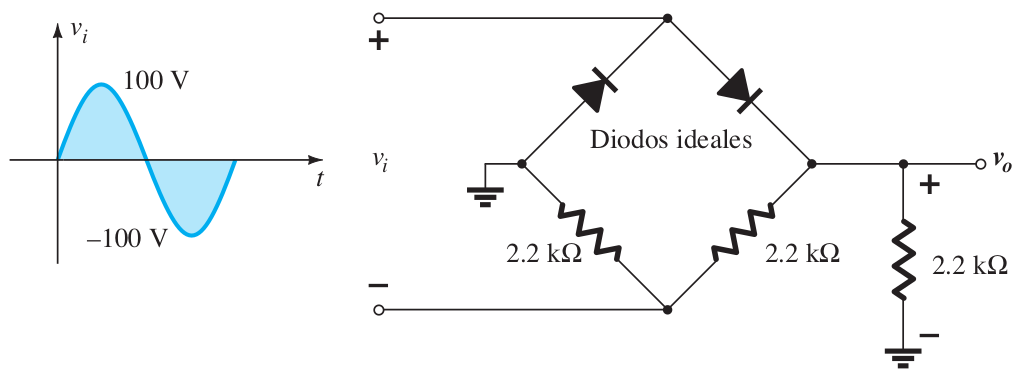
\includegraphics[scale=0.4]{c11.png} 
\end{minipage}

\begin{minipage}{8cm}
b)

	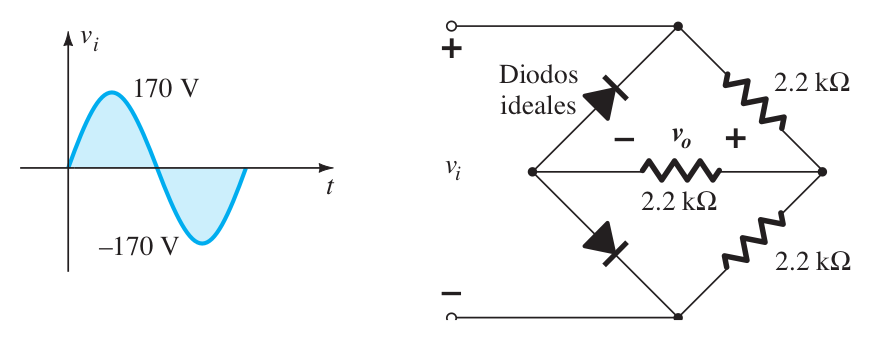
\includegraphics[scale=0.45]{c12.png}
\end{minipage}

\begin{minipage}{8cm}
	c), d)
	
	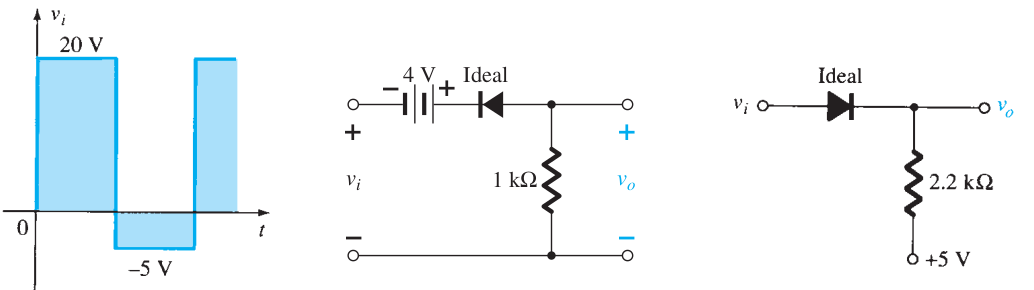
\includegraphics[scale=0.45]{c13.png}
\end{minipage}

\begin{minipage}{8cm}
	e), f)
	
	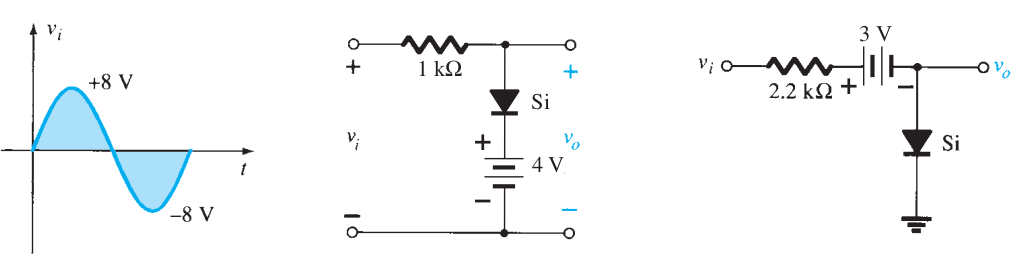
\includegraphics[scale=0.45]{c14.png}
\end{minipage}
\\

2- La figura muestra un esquema simplificado del regulador de una fuente conmutada. El capacitor y el inductor almacenan energía cuando el conmutador se encuentra encendido (se comporta como un cortocircuito) y cuando se apaga el conmutador (abierto) proveen energía a la carga. 
El conmutador se enciende con una frecuencia establecida pero el \% del tiempo en cada estado depende del valor de $V_{OUT}$.

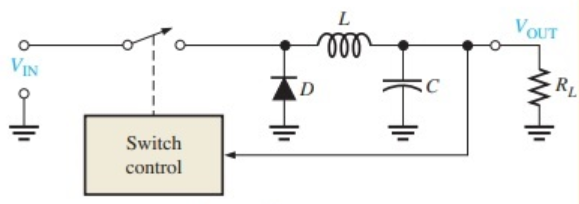
\includegraphics[scale=0.5]{c2.png}

Diga que función tiene el diodo y a partir de cuales parámetros debe ser escogido un diodo para utilizar en este circuito. \\

3- La amplitud de una portadora con frecuencia $\omega_c$ fue modulada por una señal $x(t)$ obteniéndose (la figura ilustra el proceso) $x_c(t)=A_c[1+\mu x(t)]\cos(\omega_ct)$, donde $A_c$ es la amplitud de la portadora y $\mu$ es una constante real positiva menor que 1.

\begin{minipage}{8cm}
a) Mencione posibles operaciones y/o circuitos a implementar para recuperar $x(t)$ a partir de $x_c(t)$.\\

b) La figura muestra una red compuesta por resistores, capacitores y un diodo conocida como detector de envolvente. ¿Si $x_c(t)$ se conecta a la entrada de la red qué se obtendría en $v$ y $v_o$? Realice una simulación en la cual se puedan ajustar los valores de $R1$, $R2$, $C1$, $C2$ y muestre el comportamiento de $v$ y $v_o$.

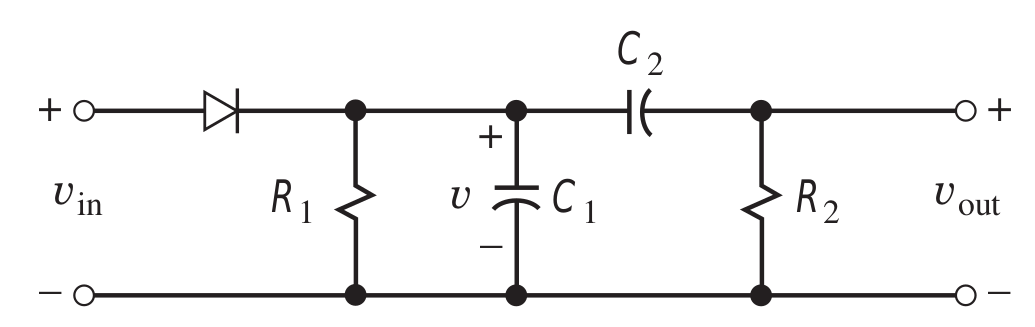
\includegraphics[scale=0.22]{c3.png}
\end{minipage}
\begin{minipage}{8cm}
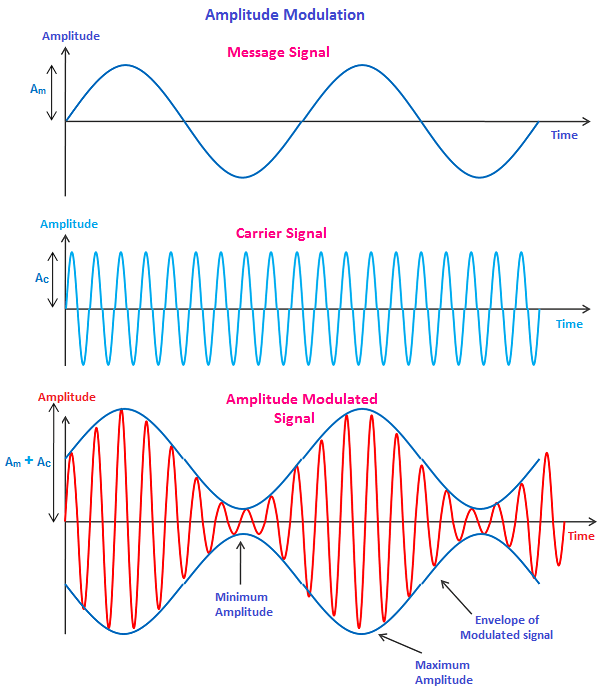
\includegraphics[scale=0.45]{c3_guide.png}
\end{minipage}

4- Diseñe un sujetador que realice la función indicada en la figura:

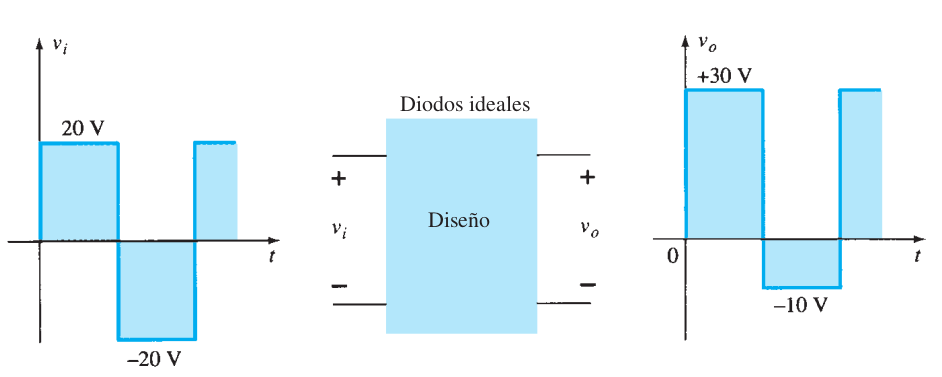
\includegraphics[scale=0.5]{c4.png}

\end{document}